% JuliaCon proceedings template
\documentclass{juliacon}
\usepackage{url}
\setcounter{page}{1}

\usepackage{amsmath}

\begin{document}

% **************GENERATED FILE, DO NOT EDIT**************

\title{Rembus: A Messaging System in Julia}

\author[1]{Attilio Donà}
\affil[1]{IT Architect, Fibercop, Trento, Italy}

\keywords{Julia, CBOR, RPC, Publish/Subscribe, Microservices architecture, Edge Computing, IoT}

\hypersetup{
pdftitle = {Rembus: A Messaging System in Julia},
pdfsubject = {JuliaCon 2022 Proceedings},
pdfauthor = {Attilio Donà},
pdfkeywords = {Julia, CBOR, RPC, Publish/Subscribe, Microservices architecture, Edge Computing, IoT},
}



\maketitle

\begin{abstract}

Rembus.jl is a Julia package designed to simplify the development of
distributed, data-intensive, and fault-tolerant applications.
By providing streamlined tools for handling complex data workflows and resilient
operations across distributed systems, Rembus.jl serves as an effective messaging
bus, ideal for high-performance computing and large-scale data processing tasks.
One of the main goals of Rembus.jl is to facilitate seamless and efficient
communication with constrained IoT microprocessors, opening avenues
for edge computing and real-time data interaction across microservices and IoT
networks.

\end{abstract}

\section{Statement of need}

Rembus.jl is a Julia~\cite{bezanson2017julia} package specifically designed to
support scalable and resilient data workflows. It provides seamless mechanisms
for publish/subscribe (Pub/Sub) and request/response (RPC) communication patterns,
making it an ideal solution for complex, data-driven applications in domains such
as edge computing, distributed systems, and high-performance data analytics.
\vskip 6pt

The landscape of messaging frameworks is diverse, encompassing established systems
like MQTT~\cite{MQTT}, gRPC~\cite{gRPC}, Kafka~\cite{Kafka}, RabbitMQ~\cite{RabbitMQ},
and NATS~\cite{NATS}, each optimized for specific use cases such as high-throughput
processing or real-time interactions. However, these frameworks often lack one
or more critical features necessary for scientific and data-intensive computing:

 \begin{itemize}
  \item \textbf{Dual Communication Styles}: Support for both Pub/Sub and RPC patterns within a unified framework.
  \item \textbf{Serialization Abstraction}: Eliminating the need for application-layer serialization logic.
  \item \textbf{Optimization for Scientific Data}: Native support for handling large-scale, structured scientific data efficiently.
  \item \textbf{Fault-Tolerant Abstractions}: Built-in mechanisms for automatic recovery from application and network failures.
  \item \textbf{Ease of Use}: A simplified API that reduces the learning curve and accelerates setup.
 \end{itemize}
  
 Rembus.jl was created with the conviction that a tightly integrated messaging
 framework, leveraging Julia’s strengths in scientific computing and offering an
 intuitive API, can revolutionize the field of distributed, data-intensive, and
 fault-tolerant applications. Its unique combination of features positions it as
 a game changer for researchers and developers who require both powerful
 data-handling capabilities and minimal overhead in building distributed systems.

\section{Key Features of Rembus.jl}\label{key-features-of-rembus.jl}

The main features that make Rembus.jl highly suited for applications requiring
reliable and responsive communication across geographically distributed
resources are:

\begin{itemize}
\item
  \textbf{CBOR Encoding}: Supports CBOR \cite{CBOR} (Concise Binary
  Object Representation), which provides compact data encoding,
  optimizing network efficiency and minimizing latency in distributed
  settings.
\item
  \textbf{RPC (Remote Procedure Calls)}: Allows services to invoke
  methods on remote systems with minimal overhead, ensuring efficient
  communication and interaction across distributed nodes.
\item
  \textbf{Publish/Subscribe Model}: Implements a publish/subscribe
  messaging model, allowing components to interact through topics,
  reducing direct dependencies between services and improving
  scalability.
\item
  \textbf{Microservices Compatibility}: Enables integration within
  microservices architectures, supporting modular, maintainable, and
  highly decoupled systems.
\item
  \textbf{DataFrames support}: DataFrames are efficiently encoded and
  may be moved between application implemented in different languages: a
  Julia DataFrame may be decoded as a pandas DataFrame, a Polars
  DataFrame or a tabular object in a language that implements the Arrow
  format~\cite{Arrow}.
\item
  \textbf{Fault tolerance}: The realiability aspects are demanded to
  Visor.jl \footnote{https://github.com/cardo-org/Visor.jl}: an Erlang
  inspired supervision model \cite{Erlang} for designing a hierarchy of
  Julia tasks that may be started, stopped and restarted in case of
  unexpected application faults or network connectivity issues.
\end{itemize}

Rembus.jl offers essential building blocks for designing and assembling the topology of a
distributed application tailored to your needs.
\vskip 6pt

The network topology of distributed applications depicted in Figure~\ref{fig:mesh}
is intentionally designed as a complex mesh of distributed applications to
demonstrate Rembus's compositional capabilities.
In practice, typical distributed applications are often organized in simpler
layouts, such as hub-and-spoke or client-server architectures.
\vskip 6pt

The following chapters will provide various code examples
demonstrating how to implement the connectivity patterns commonly found in distributed
architectures.
First, we will introduce the key concepts necessary to understand the API design. Then, we
will explore basic connectivity models through concise, minimal working examples that
highlight the core features offered by Rembus.

\begin{figure}[t]
\centerline{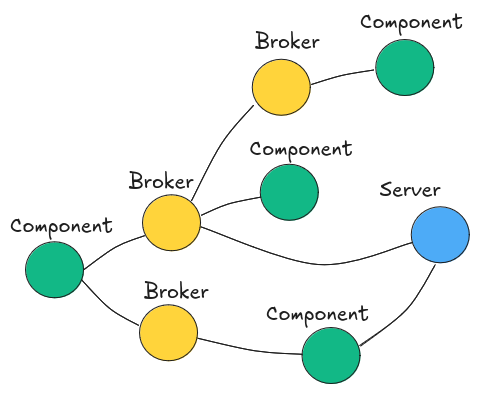
\includegraphics[width=8cm]{figures/mesh.png}}
\caption{Mesh of connected nodes using the 3 types of Rembus building blocks,
         \texttt{Component}, \texttt{Server} and \texttt{Broker}.}
    \label{fig:mesh}
\end{figure}

\section{Getting Started}\label{getting-started}

To begin using Rembus, simply add the package to your Julia environment:


\begin{lstlisting}[
  language = Julia, 
  numbers=left, 
  label={lst:getting_started} 
]
using Pkg
Pkg.add("Rembus")
\end{lstlisting}

Rembus requires no additional dependencies, infrastructure setup, or
server configuration. You can get up and running immediately with
minimal effort.
\vskip 6pt

Rembus integrates seamlessly with the Julia REPL interpreter, making it
an excellent tool for interactive use. All the code snippets in this
article are minimal working examples designed to run in REPL's
interactive mode. This feature not only supports a hands-on learning
experience but also facilitates rapid prototyping.

\section{Basic concepts}\label{basic-concepts}

Rembus provides three fundamental types of nodes---\textbf{Component},
\textbf{Server}, and \textbf{Broker}--- that serve as building blocks
for creating distributed systems using the Rembus protocol.
\vskip 6pt

A \texttt{Component} is a versatile node that connects to other nodes
and can assume multiple roles:

\begin{itemize}
\item
  \textbf{RPC Client}: Sends requests and waits for responses.
\item
  \textbf{RPC Server}: Responds to requests from other nodes.
\item
  \textbf{Pub/Sub Publisher or Subscriber}: Publishes messages to a
  topic or subscribes to receive updates.
\item
  A \textbf{Component} can combine these behaviors, enabling complex and
  dynamic roles in your system.
\end{itemize}

A \texttt{Server} is a node designed to accept connections from other nodes. It can:

\begin{itemize}
\item
  Expose methods to provide services.
\item
  Act as a source or sink for a stream of messages.
\item
  Make RPC requests to other nodes.
\end{itemize}

A \texttt{Broker} facilitates communication by routing RPC and Pub/Sub
messages between connected nodes. It can:

\begin{itemize}
\item
  Accept connections from \texttt{Components}.
\item
  Connect to \texttt{Servers}.
\end{itemize}

\subsection{API Design}\label{api-design}

The Rembus API revolves around \texttt{Component},
\texttt{Broker} and \texttt{Server}, streamlining the complexities of network
programming and fault tolerance for developers. By abstracting away the
underlying intricacies, the API enables you to concentrate on designing and
deploying robust distributed applications with ease.

\vskip 6pt

The following constructors return a handle for interacting with a node,
equipped with a supervised process that automatically handles faults and
network connectivity issues.

\begin{itemize}
\item
  \texttt{component(url)}: Creates a \texttt{Component}.
\item
  \texttt{server(;args)}: Creates a \texttt{Server}.
\item
  \texttt{broker(;args)}: Creates a \texttt{Broker}.
\end{itemize}

See Code~\ref{lst:server1}, which demonstrates creating a
\texttt{Server} and adding a service to it.

\subsection{Low-Level Connection
Management}\label{low-level-connection-management}

For applications that require custom fault-handling logic, Rembus offers a
low-level, unsupervised \texttt{connect()} API as an alternative to the
\texttt{component()}-based handle.
\vskip 6pt

Unlike the supervised \texttt{component()} API, which automatically manages
connection recovery, the \texttt{connect()} API delegates fault recovery
entirely to the application logic. This provides greater flexibility for
developers who need fine-grained control over connection management in their
distributed systems.

\subsection{Connection Parameters}\label{connection-parameters}

A \texttt{Component} connecting to a \texttt{Server} or \texttt{Broker}
can:

\begin{itemize}
\item
  Specify a \textbf{name} or remain anonymous.
\item
  Choose a transport \textbf{protocol}.
\item
  Provide the \textbf{address} and \textbf{port} of the listening node.
\end{itemize}

These parameters form a URL, which is passed to the \texttt{component}
constructor. For example, the URL \texttt{ws://localhost:9000/foo}
specifies:

\begin{itemize}
\item
  The \textbf{WebSocket} protocol (\texttt{ws}).
\item
  A connection to a node on the \textbf{local machine} at port
  \textbf{9000}.
\item
  A \texttt{Component} named \textbf{foo}.
\end{itemize}

Anonymous connections omit the path part of the URL.
\vskip 6pt

Rembus defines default values for common parameters:

\begin{itemize}
\item
  \textbf{Protocol}: \texttt{ws} (WebSocket).
\item
  \textbf{Address}: \texttt{127.0.0.1} (localhost).
\item
  \textbf{Port}: \texttt{8000}.
\end{itemize}

These defaults can be overridden using environment variables, allowing
the string \texttt{"foo"} to act as a valid connection identifier.
\vskip 6pt

It is important to note that in Rembus, the URL path (see Figure~\ref{fig:url})
serves to identify the connecting \texttt{Component}, rather than representing a
resource endpoint on the server as is common in REST architectures.

\begin{figure}[t]
  \centerline{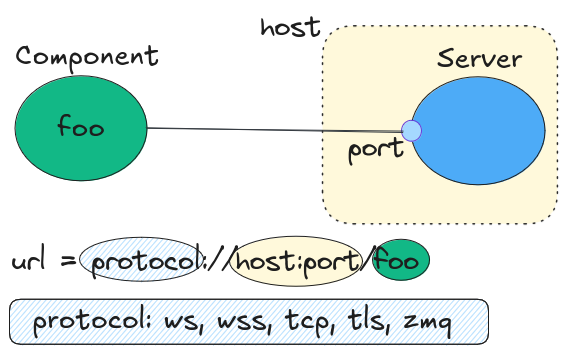
\includegraphics[width=6cm]{figures/cid.png}}
  \caption{A connection between nodes is defined by an URL.}
  \label{fig:url}
\end{figure}


\newpage{}

\section{Component-Server model}\label{component-server-model}

The foundation of the service-oriented architecture is made of one \texttt{Server}
node that provides one or more services to many clients.

Code~\ref{lst:server1} example implements a WebSocket server listening on
port \texttt{9001} and exposing the method \texttt{sum}.

\begin{lstlisting}[
    language = Julia, 
    numbers=left, 
    label={lst:server1}, 
    caption={A \texttt{Server} exposing the service \texttt{sum}.}
]
using Rembus

sum(x, y) = x + y

rb = server(ws=9001)
expose(rb, sum)
forever(rb)
\end{lstlisting}

\vskip 6pt

Code~\ref{lst:client} is a client \texttt{Component} that connects to WebSocket
port \texttt{9001} and makes a request to the remote node that exposes the
service \texttt{sum}.

\begin{lstlisting}[
    language = Julia, 
    numbers=left, 
    label={lst:client}, 
    caption={A \texttt{Component} that requests the RPC service \texttt{sum}.}
]
using Rembus

rb = component("ws://localhost:9001/my_node")
result = rpc(rb, "sum", [1, 2])
\end{lstlisting}

\section{Component-Broker model}\label{component-broker-model}

The Component-Broker model centers around a central node, the \texttt{Broker},
to which other nodes, known as \texttt{Components}, connect. The \texttt{Broker}
acts as a decoupling hub, routing messages between connected \texttt{Components},
enabling efficient and scalable communication.
\vskip 6pt

Code~\ref{lst:broker}, Code~\ref{lst:subscriber} and Code~\ref{lst:client} illustrate a
simple example of a \texttt{Broker} that facilitates
communication between two \texttt{Components}, one acting as a producer and the
other as a consumer of messages. The producer publishes a \texttt{DataFrame}
object to a logical topic channel. Upon subscribing to this topic, the consumer
receives the message with the \texttt{DataFrame} as its payload.
\vskip 6pt

In this scenario, there is only one subscribed \texttt{Component}; however, the
Pub/Sub communication style inherently supports a one-to-many model. A single
published message can be broadcast to multiple subscribed \texttt{Components},
enabling efficient message dissemination.
\vskip 6pt

A \texttt{Broker}'s role is solely to route messages between \texttt{Components}.
For instance, the example in Code~\ref{lst:broker} demonstrates how to start a
\texttt{Broker} that accepts connections from \texttt{Components},
enabling seamless message exchange.

\begin{lstlisting}[
    language = Julia, 
    numbers=left, 
    label={lst:broker}, 
    caption={A \texttt{Broker} that speaks WebSocket, plain TCP and ZeroMQ protocols.}
]
using Rembus
broker(ws=8000, tcp=8001, zmq=8002)
\end{lstlisting}

A \texttt{Component} that wants to receive messages published to a topic
must first define a method that behaves as a callback when a message is
received and then declare its interest in the topic with the
\texttt{subscribe} API.

\begin{lstlisting}[
    language = Julia, 
    numbers=left, 
    label={lst:subscriber}, 
    caption={A \texttt{Component} that consumes published messages.}
]
using Rembus

function my_topic(df)
  @info "received dataframe:" df
end

rb = component("my_consumer")
subscribe(rb, my_topic)
forever(rb)
\end{lstlisting}

A \texttt{Component} sends messages with the \texttt{publish} method.
\vskip 6pt

The first argument of \texttt{publish} is the node handle and the second
argument is the topic name.
\vskip 6pt

The third argument may be a value or a list of values. In the first case
the subscribed method expects a single argument, otherwise the list of
values maps with the arguments list of the subscribed method.

\begin{lstlisting}[
    language = Julia, 
    numbers=left, 
    label={lst:publisher}, 
    caption={An anonymous \texttt{Component} that publishes a DataFrame to topic \texttt{my\_topic}.}
]
using Rembus
using DataFrames

df = DataFrame(:a=>[1,2], :b=>["x", "y"])
rb = component()
publish(rb, "my_topic", df)
\end{lstlisting}

Note that in the above example an anonymous \texttt{Component} is
created with the zero args \texttt{component} constructor.

\section{Server-Broker model}\label{server-broker-model}

In this model, a \texttt{Broker} establishes connections to \texttt{Server} nodes, rather
than accepting connections from \texttt{Components}.
As a result, the \texttt{Broker} is no longer a connectable entity that requires a fixed DNS
name or static IP address.
\vskip 6pt

This design enables intelligent load balancing—for instance, multiple \texttt{Brokers} can
dynamically connect to \texttt{Server} nodes based on messaging load, all while remaining
transparent to the server application, see Figure~\ref{fig:server-broker}.

\begin{figure}[t]
  \centerline{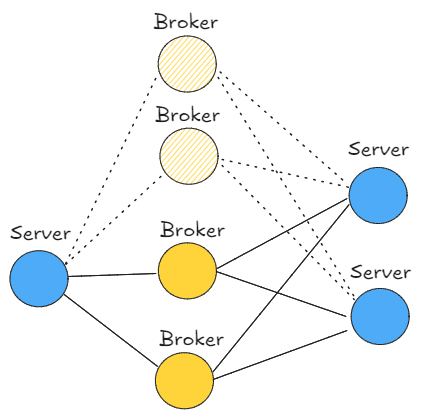
\includegraphics[width=6cm]{figures/server-broker.png}}
  \caption{Load balancing is achieved through multiple \texttt{Brokers} that establish
           connections to \texttt{Server} nodes. Dashed \texttt{Brokers} represent those
           that can be dynamically added to enhance system redundancy or load-balancing
           capacity. Since the \texttt{Broker} functions as a connector, scaling can be
           performed transparently without affecting the \texttt{Server} nodes.}
  \label{fig:server-broker}
\end{figure}

The nodes in Code~\ref{lst:server1}, Code~\ref{lst:server2}, Code~\ref{lst:broker-mobile} and
Code~\ref{lst:client-frontend} illustrate a connectivity pattern where a \texttt{Broker} acts
as a smart proxy for a group of \texttt{Servers}. In this configuration, the \texttt{Component}
is decoupled from the \texttt{Servers}.
\vskip 6pt

Additionally, the example demonstrates a scenario where a node handle is required by an
exposed method. Specifically Code~\ref{lst:server2} starts a \texttt{Server} node and
exposes the method \texttt{summary} that needs to make an RPC request to
another node before returning a response.
\vskip 6pt

To enable the injection of the node handle into the callback method
\texttt{summary} the \texttt{inject} API must be used. See
Section~\ref{sec-inject} for more details.

\begin{lstlisting}[
    language = Julia, 
    numbers=left, 
    label={lst:server2}, 
    caption={A \texttt{Server} node that bases its response on a RPC request to another \texttt{Server}, the
    node in Code~\ref{lst:server1}.}
]
using Rembus

function summary(ctx, rb, x, y)
  result = rpc(rb, "sum", [x,y])  
  return "sum is $result"
end

handle = server(ws=9002)

inject(handle)
expose(handle, summary)
forever(handle)
\end{lstlisting}


A \texttt{Broker} node that needs to establish connections with \texttt{Server} nodes must
be configured with a set of URLs identifying those nodes.
\vskip 6pt
Each \texttt{Server} intended for connection with the \texttt{Broker} must be set up using
the \texttt{add\_node} API. Refer to Code~\ref{lst:broker-mobile} for an example.
\vskip 6pt
The \texttt{add\_node} API can also be used to connect a \texttt{Broker} to another
\texttt{Broker}. This advanced feature, primarily related to channel bundling, should be
explored further if relevant use cases arise.

\begin{lstlisting}[
    language = Julia, 
    numbers=left, 
    label={lst:broker-mobile}, 
    caption={A \texttt{Broker} that connects to \texttt{Server} nodes.}
]
using Rembus

rb = broker(wait=false)
add_node(rb, "ws://:9001/server_1")
add_node(rb, "ws://:9002/server_2")
forever(rb)
\end{lstlisting}

Finally Code~\ref{lst:client-frontend} shows a RPC client that
requests the \texttt{summary} service from the broker, which in turn will route the
request to the server in Code~\ref{lst:server2}.

\begin{lstlisting}[
    language = Julia, 
    numbers=left, 
    label={lst:client-frontend}, 
    caption={A RPC client that requests the service \texttt{summary}.}
]
using Rembus

rb = component("my_client")
result = rpc(rb, "summary", [1, 1])
\end{lstlisting}


\begin{figure}[t]
  \centerline{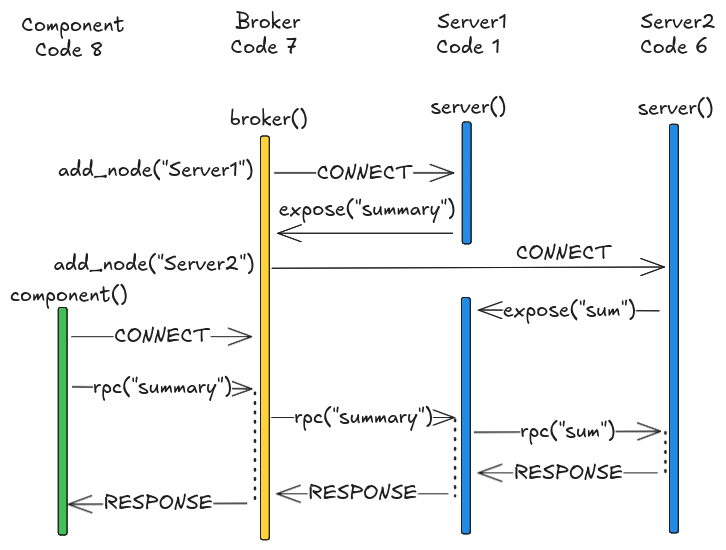
\includegraphics[width=8cm]{figures/server-broker-example.png}}
  \caption{Sequence diagram of the events occuring in the system made of 
          one \texttt{Component} (Code~\ref{lst:client-frontend}), two
          \texttt{Servers} (Code~\ref{lst:server1} and (Code~\ref{lst:server2}))
          and one \texttt{Broker} (Code~\ref{lst:broker-mobile}).}
      \label{fig:server-broker-example}
  \end{figure}

The interactions between nodes are illustrated in Figure~\ref{fig:server-broker-example}.
This configuration ensures that the \texttt{Component} remains unaware of the
\texttt{Servers}' locations.

\section{Multiplexing}\label{multiplexing}

A \texttt{Component} can utilize a pool of connections to interact with multiple
\texttt{Brokers} or \texttt{Servers}.

This capability addresses the single point of failure inherent to a single \texttt{Broker},
enabling high-availability configurations.
\vskip 6pt

Multiplexing a \texttt{Component} is also valuable for implementing advanced functionalities,
such as patterns requiring multiple responses—for example, the majority-vote mechanism.
\vskip 6pt

The behavior of multiplexing is governed by the following policies:

\begin{itemize}
  \item \texttt{firstup\_policy}: Uses the first available connection that is active.
  \item \texttt{roundrobin\_policy}: Distributes messages across connections in a round-robin fashion.
  \item \texttt{lessbusy\_policy}: Selects the connection with the fewest outstanding requests.
  \item \texttt{all\_policy}: Sends the message to all connections and, in the case of RPC, expects multiple responses.
\end{itemize}

\begin{lstlisting}[
    language = Julia, 
    numbers=left, 
    label={lst:multiplexing}, 
    caption={A \texttt{Component} that connects to a pool of \texttt{Brokers} in a high-availability scenario.}
]
using Rembus

rb = component([
    "ws://broker1",
    "ws://broker2", 
    "ws://broker3"
])

# By default the policy is firstup_policy.
# The following line may be commented out.
firstup_policy(rb)

# If host1 is up all requests get routed to it.
result = rpc(rb, "my_service", [arg1, ...])
\end{lstlisting}

\section{Pub/Sub Quality of Service}

A Pub/Sub message gets delivered to all subscribed nodes and it is send-only: the publisher
does not expect a response. 

The type of delivery guarantee between the publisher and
the subscriber is defined by the following levels of Quality of Service:

\begin{itemize}
    \item \emph{QOS0}: At most once.
    \item \emph{QOS1}: At least once.
    \item \emph{QOS2}: Exactly once.
\end{itemize}

At most once (\emph{QOS0}) is the fire and forget sending paradigm, it is the most efficient way of
publishing messages but there is no guarantee of message reception by the subscribers.
\vskip 6pt
At least once (\emph{QOS1}) guarantees that the message will be delivered to the subscribers
but it is possible that duplicated messages may be received.
\vskip 6pt
Exactly once (\emph{QOS2}) guarantees that exactly one copy of the message will be delivered
to the subscribers. This quality setting is the most impactful from a performance point of view.
\vskip 6pt
The \emph{publish()} argument keyword \emph{qos} set the Quality of Service requested. It defaults to \emph{QOS0}.
\vskip 6pt
Code~\ref{lst:publish-qos2} shows how to publish a message with QOS "exactly once". 

\begin{lstlisting}[
    language = Julia, 
    numbers=left, 
    label={lst:publish-qos2}, 
    caption={Publish a message with QOS2 "exactly once" guarantee}
]
using Rembus

rb = component("publisher")
publish(rb, "mytopic", ["arg1", "arg2"], qos=QOS2)

\end{lstlisting}

Figure~\ref{fig:pubsequence} shows the flows of packets involved in a message published 
with the \emph{QOS2} service level.
\vskip 6pt

For the \emph{QOS0} level the only packets are the \emph{publish} messages between publisher
and broker and between broker and subscriber. \emph{QOS1} introduces the \emph{ack} packet
and \emph{QOS2} introduces the \emph{ack2} packet. 
This gives an idea of why performances degrade as the service level increases.

\begin{figure}[t]
  \centerline{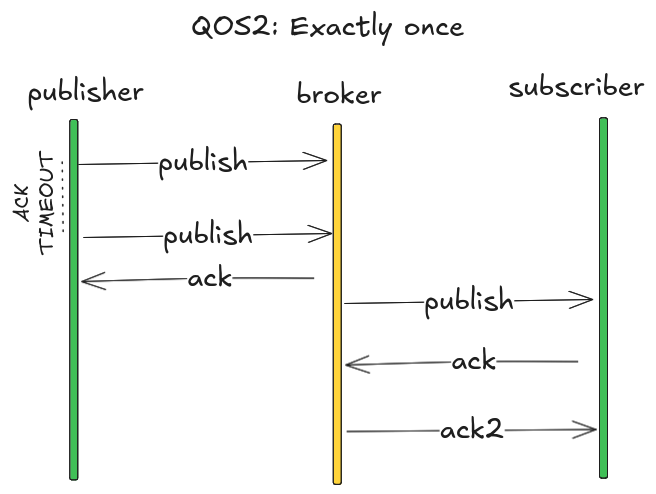
\includegraphics[width=8cm]{figures/pubsequence.png}}
  \caption{Sequence diagram for QOS2 publishing.}
      \label{fig:pubsequence}
\end{figure}
  

\section{Injecting context and node handle}\label{sec-inject}

There are cases where either it is necessary to keep state between exposed and subscribed
callback methods or to have at disposal the handle that represents the node, for example to
make RPC requests or publish messages in the body of the callback. 
\vskip 6pt

Rembus provides both these capabilities through the \texttt{inject()}
API.

\begin{lstlisting}[
    language = Julia, 
    numbers=left, 
    label={lst:inject}, 
    caption={The inject API may be used for sharing state and to injecting the node handle.}
]
using Rembus

mutable struct Context
  ...
Context() = new(...)
end

# case 1: share a state value and
# inject the node handle.
state = Context() 
inject(handle, state)

# case 2: inject only the node handle.
# In this case the state value is `Nothing`.
inject(handle)
\end{lstlisting}

When \texttt{inject} is used the subscribed and exposed methods expect
as a first argument the state value and as a second argument the node
handle, see Code~\ref{lst:inject-example}.

\begin{lstlisting}[
    language = Julia, 
    numbers=left, 
    label={lst:inject-example}, 
    caption={Example of configuring a state value to be shared among exposed/subscribed methods.}
]
using Rembus

function service_a(
  ctx, rb, name::String, count::Int
)
  ctx.state[name] += count
  publish(rb, "my_topic", name, totals)
  return fn(...)
end

function service_b(ctx, rb, name::String)
  if haskey(ctx.state, name)
    error("service_b: unknown $name")
  end
  res = rpc(rb, "service_c", name, ctx.state[name])
  return res
end

mutable struct Context
  state::Dict
  Context() = new(Dict())
end

ctx = Ctx()

handle = connect()
inject(handle, ctx)
expose(handle, service_a)
expose(handle, service_b)
\end{lstlisting}

\section{Macro-based API}\label{macro-based-api}

A macro-based API fits naturally into the language the concepts of
message streaming and RPC service requests.
\vskip 6pt

With this approach message publishing and RPC requests are executed as
method calls prefixed with the tags \texttt{@publish} and \texttt{@rpc}.

A julia function becomes an RPC service with the tag \texttt{@expose} and
a function becomes a Pub/Sub topic consumer with the tag
\texttt{@subscribe}.

\begin{lstlisting}[
    language = Julia, 
    numbers=left, 
    label={lst:macroapi}, 
    caption={The macro-based API. An RPC service is a method that is made available with
    \texttt{@expose}, a RPC request is a function call tagged with \texttt{@rpc}.
    A published message is a function call tagged with \texttt{@publish}.}
]
using Rembus

function myservice(title::String, df::DataFrame)
  val = sum(df.a)
  return "$title=$val"
end

@expose myservice

astring = "totals:"
df = DataFrame(:a=>1:100)

result = @rpc my_service(astring, df)

@publish my_topic(df)
\end{lstlisting}

\section{Http restful API}\label{http-restful-api}

Rembus implements an experimental HTTP Restful API. The RPC services are
accessible with GET methods and the Pub/Sub topics through the POST
verb.
\vskip 6pt

A GET method will return the RPC response in the HTTP response body
formatted as a JSON string.
\vskip 6pt

The HTTP API must be esplicitly activated with the \texttt{http} option,
see Code~\ref{lst:http}.

\begin{lstlisting}[
    language = Julia, 
    numbers=left, 
    label={lst:http}, 
    caption={How to enable the HTTP protocol on port \texttt{8080} alongside the Websocket
    protocol on the default port \texttt{8000}.}
]
using Rembus

broker(http=8080)

# Activate the HTTP port for a Server node.
#server(http=8080)

\end{lstlisting}

The path of the URL is the RPC service or the Pub/Sub topic and the body
of the HTTP request is a JSON formatted list of arguments.
\vskip 6pt

Basic authentication is employed for accessing protected RPC methods and
Pub/Sub topics.

\section{Security and multitenancy}\label{security-and-multitenancy}

Rembus provides cyphered connections through Secure WebSockets and TLS
protocols and supports node authentication using RSA or ECDSA
algorithms. The \texttt{Component} owns the private key, whereas the public key
must be commissioned to the \texttt{Server} and \texttt{Broker} nodes.
\vskip 6pt

There is also the less secure option to share a password between the
nodes, and this is actually the way to autenticate for HTTP clients
using the REST approach.
\vskip 6pt

Multitenancy is implemented in the \texttt{Broker} and when it is enabled Pub/Sub messages
and RPC requests are only routed between nodes belonging to the same tenant. 
\vskip 6pt

\section{Conclusion}\label{conclusion}

Rembus represents an exciting step forward in messaging technology, with Julia as its
primary supported language. A preliminary implementation for Python
\footnote{https://github.com/cardo-org/rembus.python} is already available,
and the project roadmap outlines ambitious goals, including support for additional
programming languages and the development of a lightweight C library tailored for
constrained microprocessors.
\vskip 6pt

The ability to encode and decode CBOR messages makes Rembus highly efficient for
communication, especially in IoT contexts. Its dual support for Pub/Sub asynchronous events
and synchronous RPC commands allows seamless integration with IoT devices without requiring
separate tools. This extends Julia's versatility, enabling it to serve as a robust backend
for distributed sensor networks and other connected systems.
\vskip 6pt

By bridging the gap between physical systems and Julia’s analytical and computational
strengths, Rembus unlocks new opportunities for innovation and integration. As an
early-stage project, it offers the Julia community a unique chance to contribute feedback,
helping to refine and expand its capabilities.
\vskip 6pt

With its potential to streamline distributed, data-intensive applications, Rembus could
become a cornerstone of modern software ecosystems. Community involvement will be pivotal in
shaping its evolution, ensuring it grows into a reliable, feature-rich, and widely adopted
technology.

% **************GENERATED FILE, DO NOT EDIT**************

\bibliographystyle{juliacon}
\bibliography{ref.bib}


\end{document}

% Inspired by the International Journal of Computer Applications template
